\chapter{設計流程}
\section{簡化模型}
將冰球機簡化成一個自由度,簡化後與Pong的操控相同,並分別透過2D遊戲Pong-v0與3D模擬環境CoppilaSim供強化學習訓練。

\section{機器學習訓練}
透過影像處理,過濾出擊錘與球,並將兩幀影像進行比較,透過調整環境參數與決策參數的權重,環境參數使用ReLU Function進行優化,決策參數則是透過Log probability和Softmax進行運算

\section{模擬環境}
 本研究分三大部分,第一運用OpenAI Gym裡內建編譯的ATARI 2600遊戲Pong-v0,來作為訓練環境,加上強化學習的理論,測試不同演算法以訓練出最佳化的對打系統,第二換為CoppilaSim模擬環境並套用訓練程式,成為優化的對打機電系統。第三則是透過架設伺服器與虛擬環境結合。\\
 
 利用Gym的訓練環境來測試不同的算法所得到的訓練結果,比較不同算法、參數間的差異,並找出較適合Pong game的算法、參數,循序漸進提高環境的真實程度,來減少一開始就是以實體的方式測試所帶來硬體、程式、時間和金錢等成本。\\

 將Gym的訓練環境轉換到CoppilaSim模擬環境,利用貼近真實的模擬環境來修正在純程式的架構(Gym)與真實環境間的誤差,雖然CoppilaSim模擬環境與真實環境仍有些微的落差,兩者相比CoppilaSim的環境已非常貼近真實了,拉近了虛擬與現實間的距離,提高了實用性的價值。這部分還有利用OpenCV進行影像處理並撰寫輔助對打程式來協助玩家預判球的移動路徑或彈射位置。影像處理除了應用在輔助對打上,最主要是應用在訓練強化學習所需的輸入訓練影像。\\
 
 再透過架設伺服器與虛擬環境結合:讓虛擬環境的影像透過網伺服器串流影像供使用者遠端進行操控虛擬環境的擊錘進行打球,或是提供多人進行觀看對打影像。
 \iffalse
\begin{figure}[hbt!]
\begin{center}
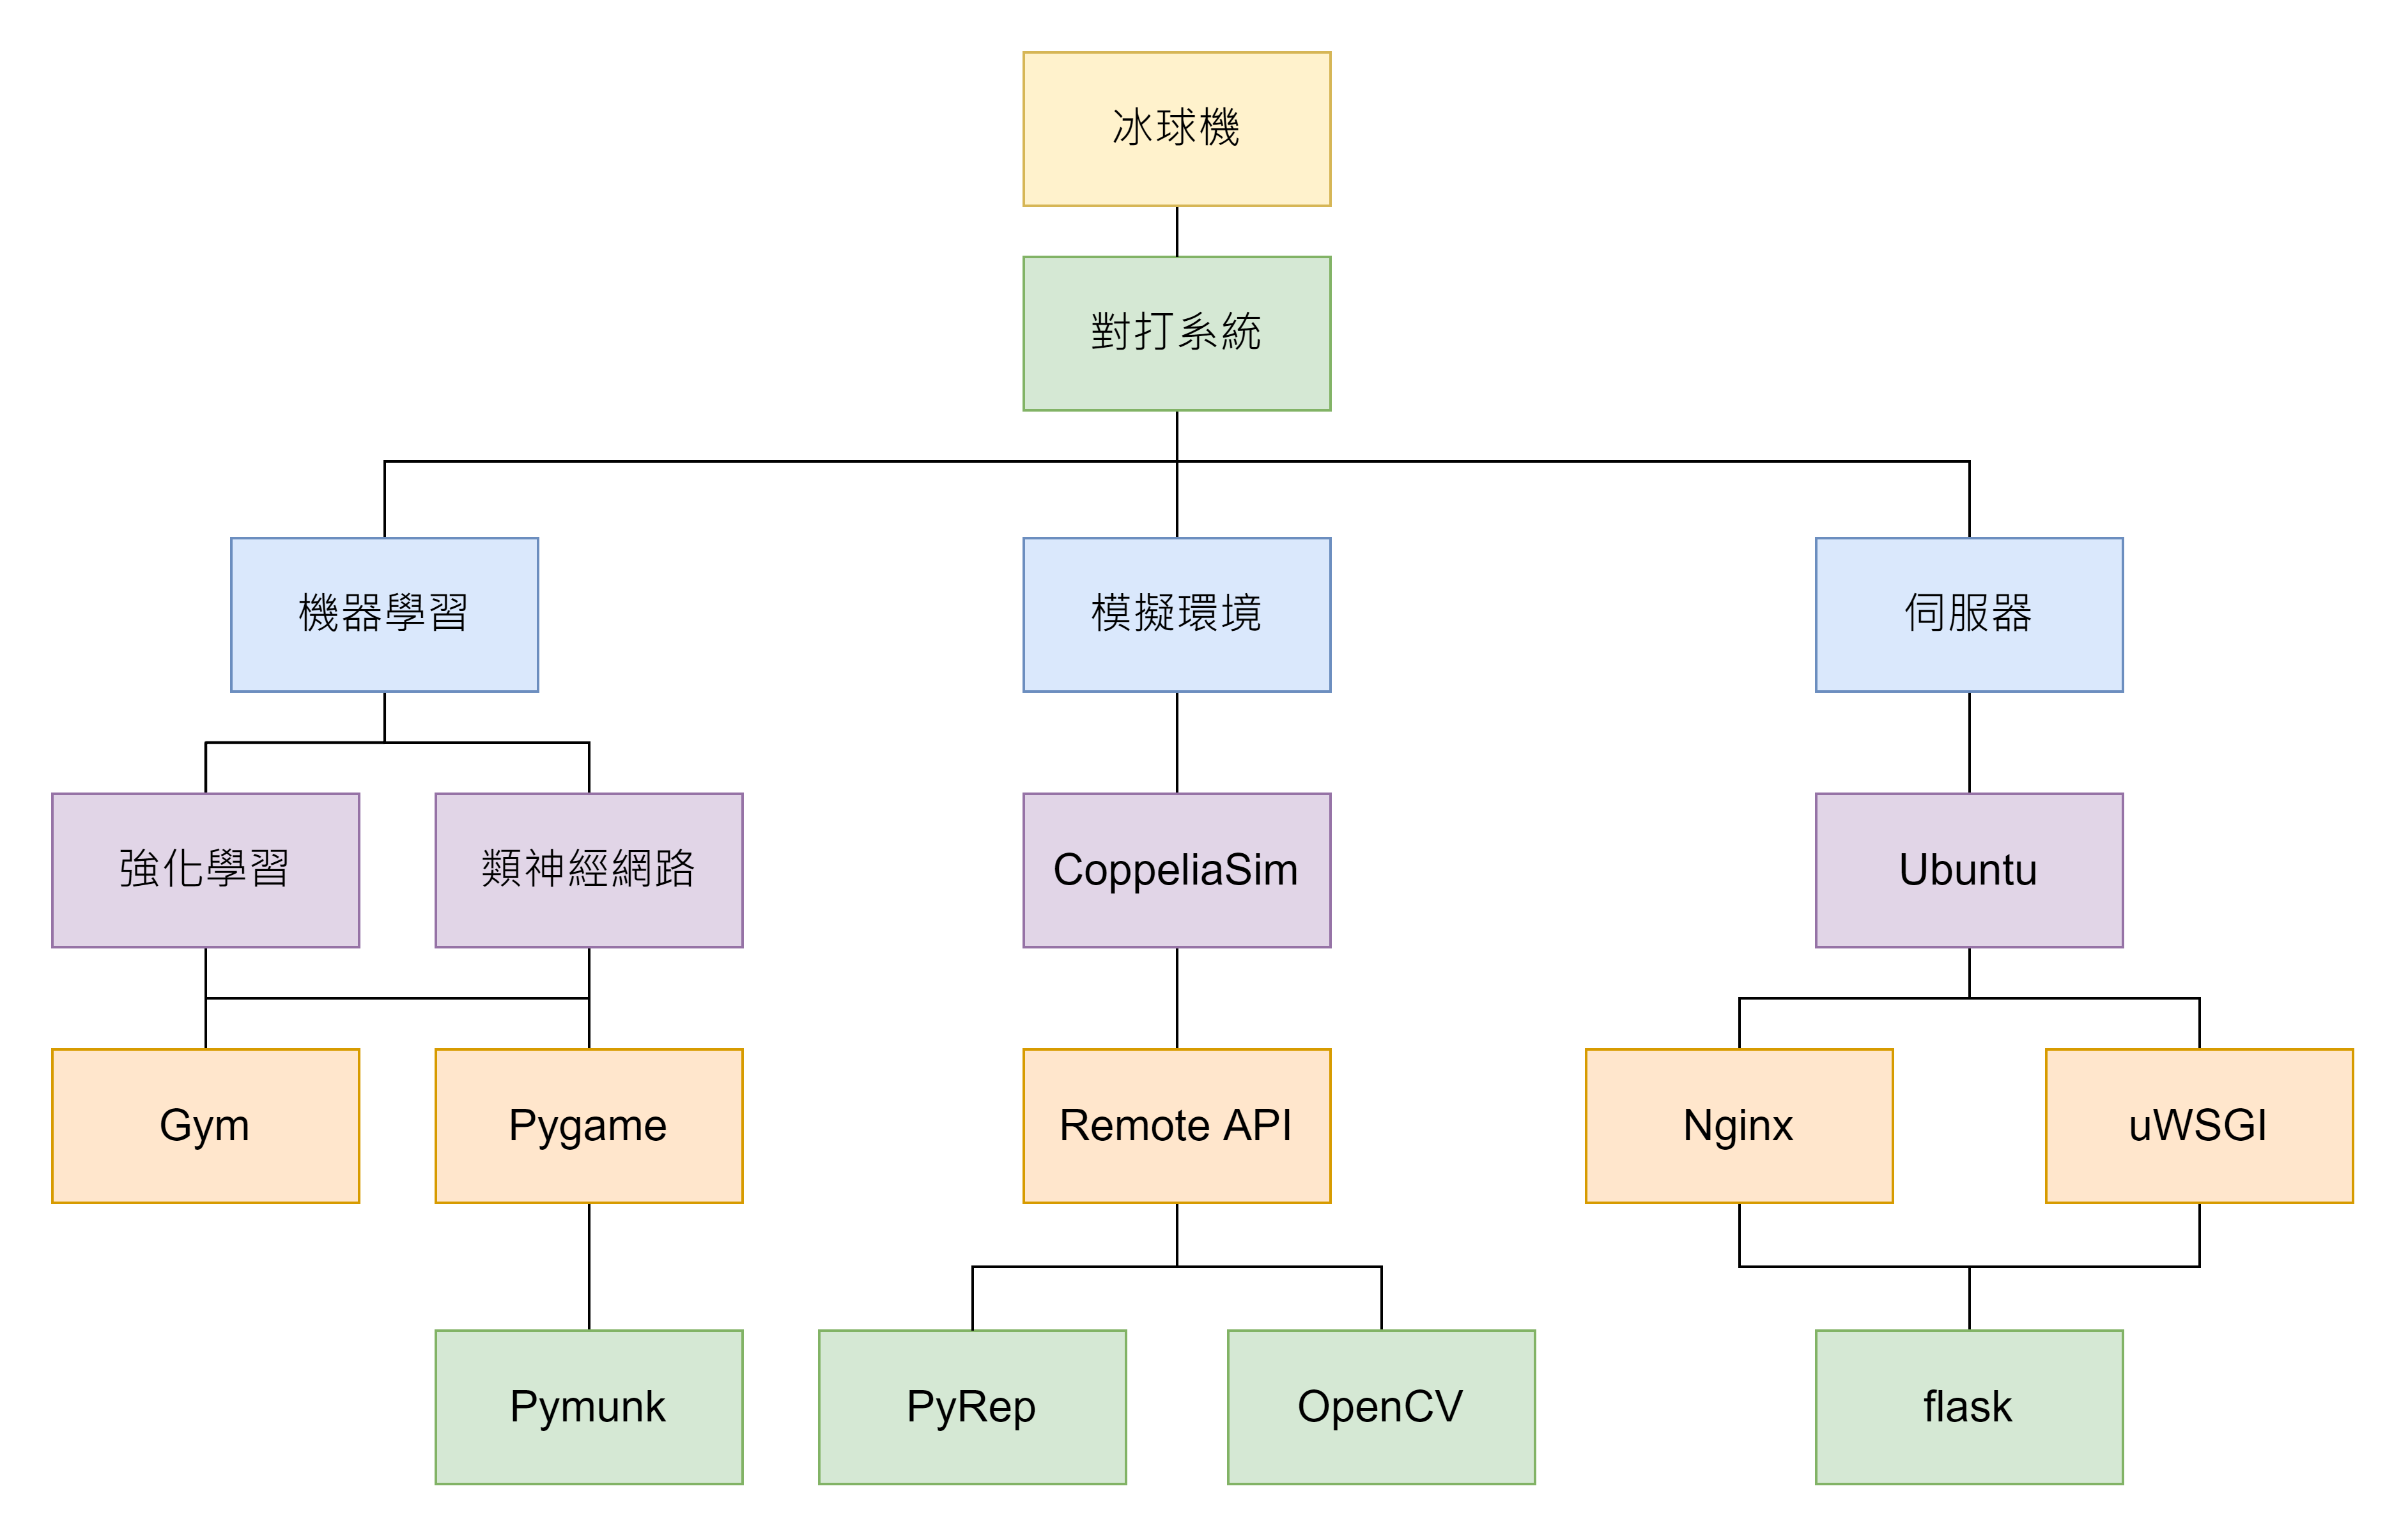
\includegraphics[width=15cm]{研究架構}
\caption{\Large 研究架構 }
\label{研究架構 }
\end{center}
\end{figure}
\fi

\section{未來展望}
此專題希望能利用現有完成的機械學習的算法,能發展成虛擬訓練,再將訓練完的機器學習應用到虛擬環境或是實體機電系統,並透過伺服器將影像串流提供玩家網頁介面進行遠端操控,同時提供多人觀看及時的比賽影像,將整個冰球機的控制和使用者間有更完善串聯,機電系統的部分達到最優化控制和虛實整合的應用。